
\subsubsection*{Allocating Gross Power Production with EBE}

\begin{figure*}[h!]
    \begin{subfigure}[c]{.495\linewidth}
    \includegraphics[width=\linewidth]{example_allocation_bus1_gross_ebe.png}
    \vspace{-40pt}
    \subcaption{}
    \label{fig:example_allocation_bus1}
    \end{subfigure}
    \begin{subfigure}[c]{.495\linewidth}
    \includegraphics[width=\linewidth]{example_allocation_bus2_gross_ebe.png}
    \vspace{-40pt}
    \subcaption{}
    \label{fig:example_allocation_bus2_gross_ebe}
    \end{subfigure}
    \caption{Power allocations for gross power injection using the EBE scheme, type \ref{gross}\ref{ebe}, for bus~1 (a) and bus~2 (b) of the example network in \cref{fig:example_network}. Bus~1 retrieves 40~MW from itself and 20~MW from bus~2. The latter in turn retrieves 60~MW from bus~1 and self supplies 30~MW.
    The sum of both net flows equals the resulting flow of $f_1=40$~MW.}
    \label{fig:example_allocation}
\end{figure*}


\begin{figure}[h]
    \centering
    \includegraphics[width=\linewidth]{example_payoff_gross_ebe.png}
    \caption{Full P2P cost allocation for the example setup shown in \cref{fig:example_network}. The payments are derived on the basis of \cref{eq:allocate_opexGeneration_detailed,eq:allocate_capexGeneration_detailed,eq:allocate_capexFlow_detailed}. Consumers at bus $n$ have to pay each generator proportional to their consumption. As we only consider one time step the proportionality applies for OPEX $\allocateopex$ and CAPEX $\mathcal{C}_{n \rightarrow i}$. As bus~1 induces a relieving flow an line~1 and therefore ``prevents`` further transmission expansion, it is rewarded proportional to the relief.}
    \label{fig:example_payoff}
\end{figure}    


\Cref{fig:example_allocation} shows the allocated transactions on basis of gross power injection for both buses 1~\&~2 separately. The resulting P2P payments are given in \cref{fig:example_payoff}.
The upper graph \cref{fig:example_allocation_bus1} shows that $A_{1 \rightarrow 1}=40$~MW at bus~1 are self-sustained. With only one generator at bus 1, consumers at bus~1 consequently pay 2k~\euro~OPEX and 22k~\euro~CAPEX to the generator~1. The remaining 20~MW come from bus~2 and induce a subflow on line 1 of $A_{\ell = 1, 1} = -20$. As this flow is in contrary direction to the total flow, it is relieving the transmission system. This translates to a congestion reward for consumers at bus~1 of $c_{\ell=1} A_{\ell = 1, 1}$~=~2k~\euro\, which is exactly the cost that had to be spent on the transmission system if bus~1 didn't induce a relieving flow, see again \cref{fig:example_payoff}. 



The lower graph \cref{fig:example_allocation_bus2_gross_ebe} illustrates the impact of consumption at bus~2. As $d_2$ is higher than $d_1$, the reception from both generators are proportionately increased as well as the OPEX and CAPEX allocations to the generators. But instead of a relieving flow, consumers at bus~2 drive the burdening flow in direction of congestion. Hence the payoff to the transmission system is positive and much higher than for bus~1.

The sum of all rows in the payoff matrix in \cref{fig:example_payoff} yields the revenues of the assets $m, \ell$. These values match their overall spending, \textit{e.g.} the total revenue of the transmission line is 4k~\euro\, which equals the cost for investments $c_{1}\,F_{1}$. The sum of all columns yields the total payment of consumers at bus $n$. For example the sum of payments of consumers at bus~1 is 36k~\euro. This is exactly the electricity price of 600~\euro/MW times the consumption of 60~MW, $\lambda_1 d_1$. \\

The fact that OPEX and CAPEX allocations are proportional to the total consumption at a bus results from optimizing one time step only. In larger optimization problems with multiple time steps the CAPEX allocation takes effect only for time steps in which one or more of the capacity constraints  \cref{eq:upper_generation_capacity_constraint,eq:lower_flow_capacity_constraint,eq:upper_flow_capacity_constraint} become binding.  

\subsubsection*{Allocating Net Power Production}

\begin{figure}[h!]
    \centering
    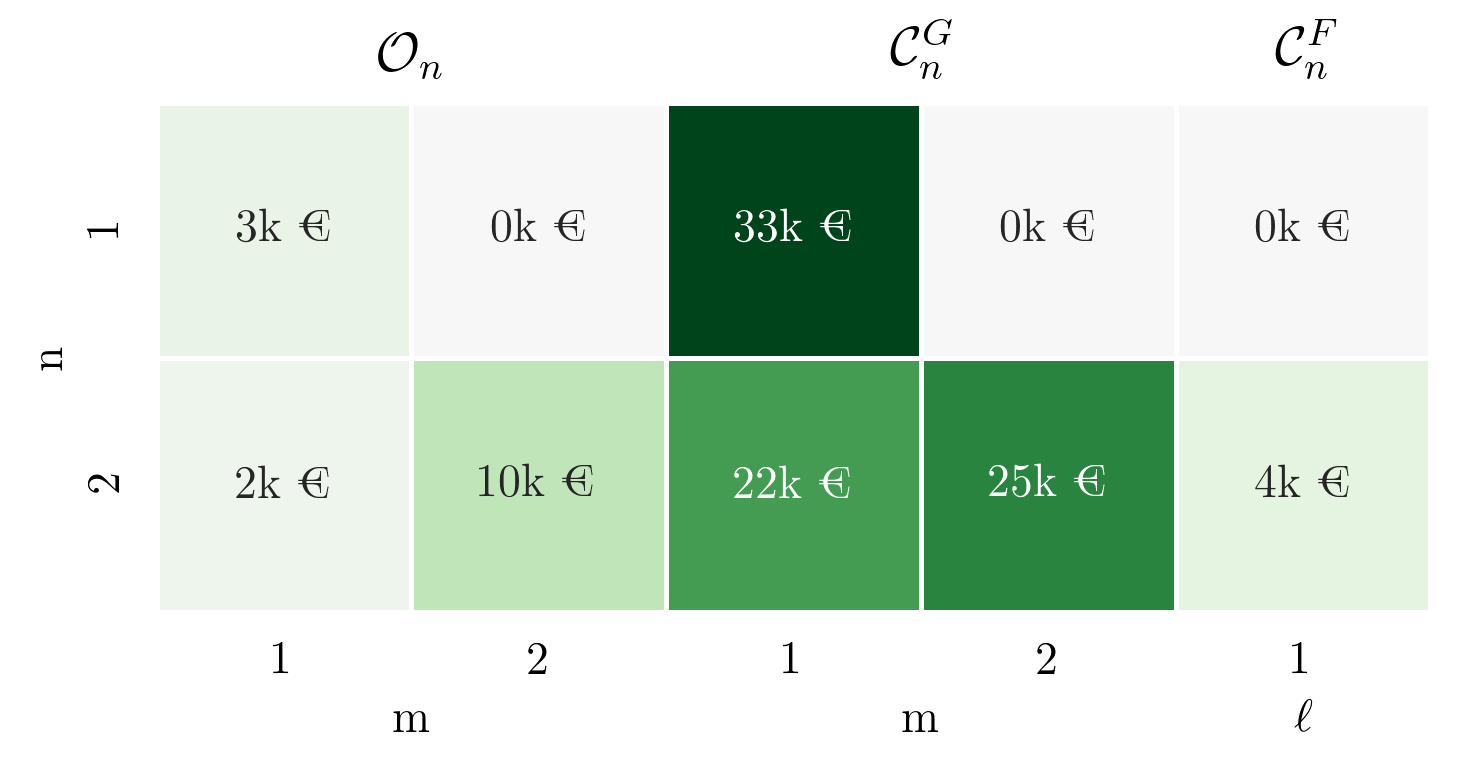
\includegraphics[width=\linewidth]{example_payoff_net_ebe.png}
    \caption{Full P2P cost allocation for the example setup shown in \cref{fig:example_network} when allocating net power injection using the EBE scheme (type \ref{net}\ref{ebe}). This leads to less and more intuitive payments.}
    \label{fig:example_payoff_net_ebe}
    \end{figure}    
% 
In contrast the to equivalent allocation of gross power production, netting out injections for each bus leads to less P2P payments. The resulting payment given in \cref{fig:example_payoff_net_ebe} builds on the allocated power flow shown \cref{fig:example_allocation_net_ebe} in \cref{sec:example_plots}. As bus~2 does not produce excess power, none of its power production is assigned to bus~1 and thus no payment of bus~1 to bus~2 allocated. Neither has bus~1 to pay fee to the transmission system as it only exports power. So, consumers at bus~1 pay to its local generator. Bus~2 in contrast bear all CAPEX for the transmission system as well as CAPEX and OPEX for generators at bus~1. 
% 
Again the cumulative payments per bus meet the nodal spending $\lmp \, \demand$. The cumulative revenues per generator and transmission line meet the all CAPEX and OPEX. Note this gives the same result as when allocating net injection with the Average Participation \ref{net}\ref{ap}.

The example shows that allocating net power injection only, reduces the number of peer-to-peer payments significantly, which leads to a much clearer pictures. The same counts for the AP scheme which we will use in the following application case.  

\subsection{Numerical Example: Power Flow Allocation of type \ref{net}\ref{ebe}}
\label{sec:example_plots}
\begin{figure}[h!]
    \begin{subfigure}[c]{.99\linewidth}
    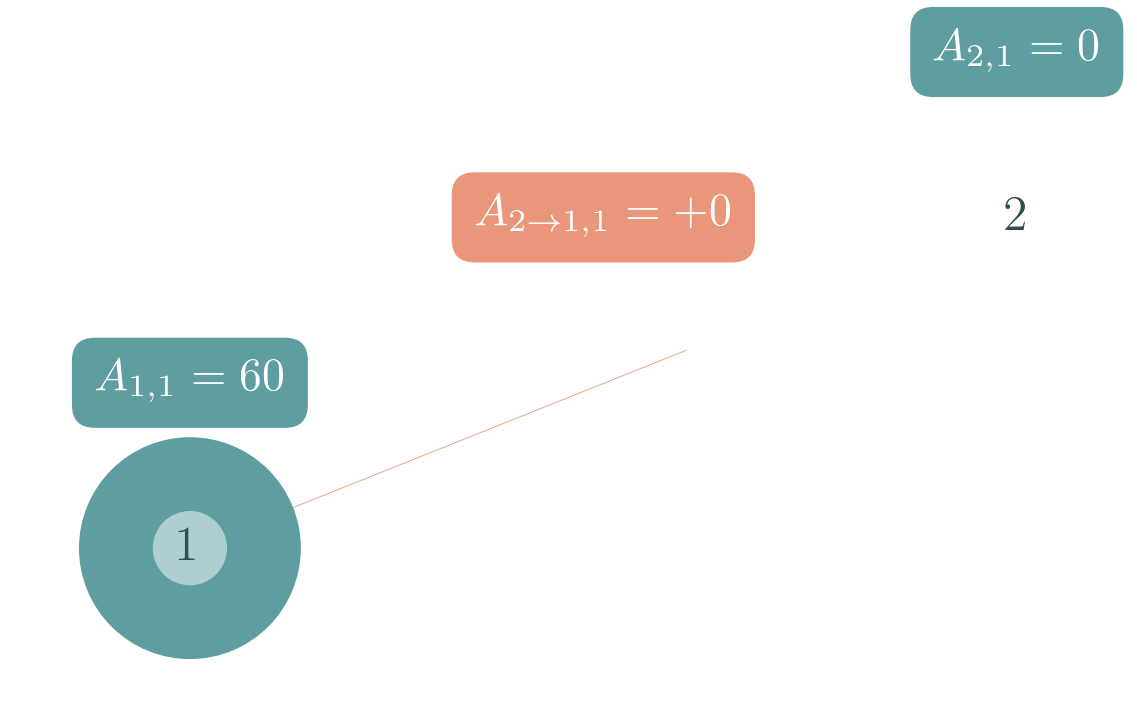
\includegraphics[width=\linewidth]{example_allocation_bus1_net_ebe.png}
    \vspace{-40pt}
    \subcaption{}
    \label{fig:example_allocation_bus1_net_ebe}
    \end{subfigure}
    \begin{subfigure}[c]{.99\linewidth}
    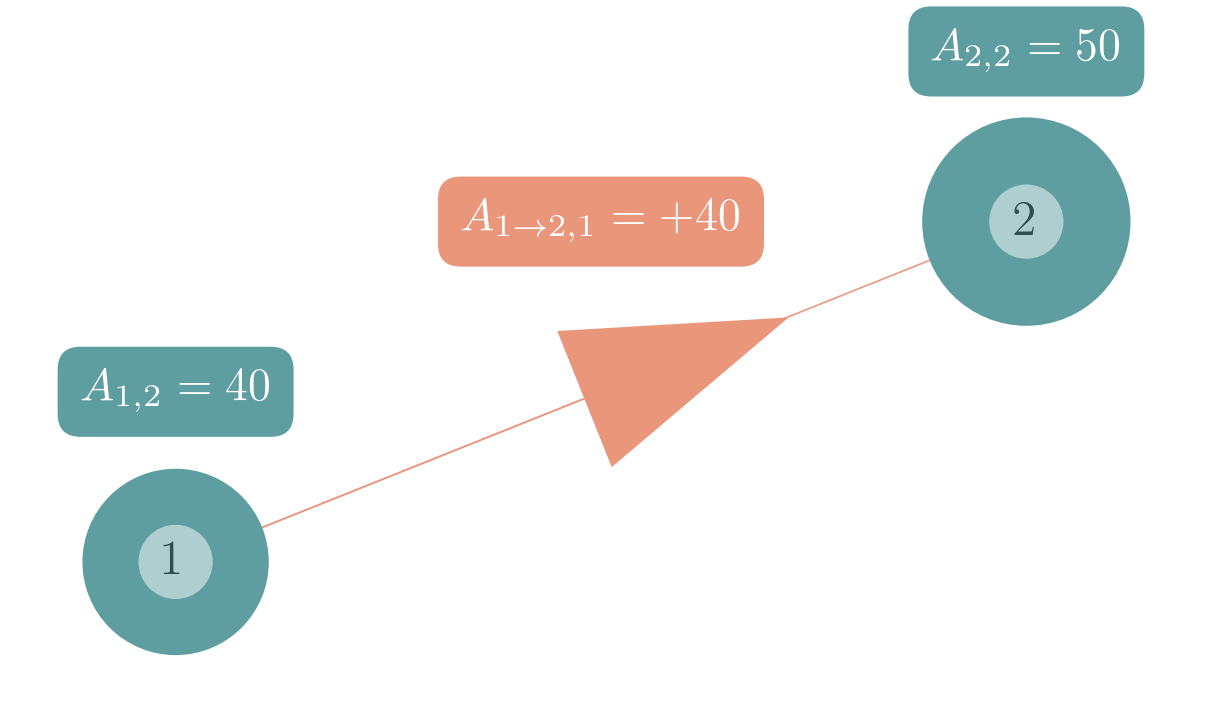
\includegraphics[width=\linewidth]{example_allocation_bus2_net_ebe.png}
    \vspace{-40pt}
    \subcaption{}
    \label{fig:example_allocation_bus2_net_ebe}
    \end{subfigure}
    \caption{Power allocations for bus~1 (a) and bus~2 (b) of the example network in \cref{fig:example_network} using equivalently allocated net power injections (scheme \ref{net}\ref{ebe}). Bus~1 retrieves 60~MW from itself and nothing from bus~2. The latter in turn retrieves 40~MW from bus~1 and self supplies 50~MW. The P2P trades are less in number and more intuitive then with allocating gross flow.}
    \label{fig:example_allocation_net_ebe}
\end{figure}
